\begin{frame}
    \frametitle{Python}
    \centering
    
\includegraphics[scale=0.06]{Bin/python_logo.png}

    \vspace{1cm}
    \pause

    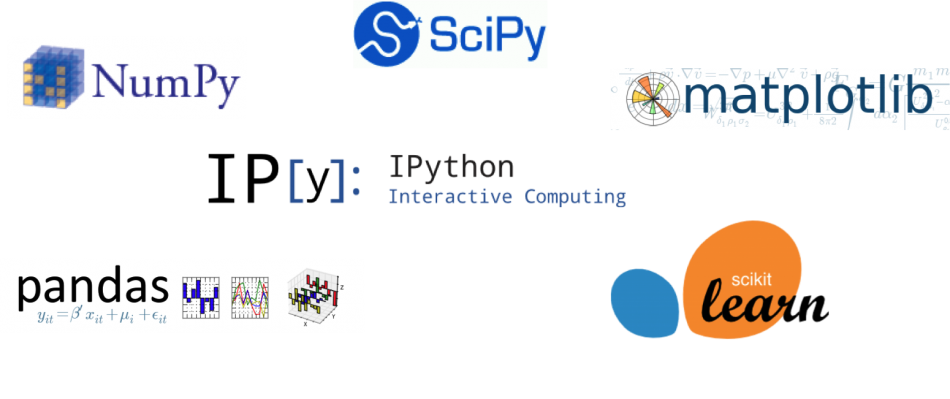
\includegraphics[scale=0.3]{Bin/python_libraries.png}

\end{frame}



\begin{frame}
    \centering
    
    \begin{multicols}{2}
        {\Large \textbf{\href{https://flit.readthedocs.io/en/latest/upload.html\#using-pypirc}{Flit}}}
    
        \vspace{0.8cm}
        \textit{Initialising}

        \vspace{0.5cm}
        \textit{Packaging}

        \vspace{0.5cm}
        \textit{Publishing}

        \columnbreak
        \pause        
        {\Large \textbf{\href{https://pypi.org/}{PyPI} \& \href{https://test.pypi.org/}{TestPyPI}}}

        \vspace{0.5cm}

        
\includegraphics[scale=0.1]{Bin/pypi_logo.png}
    \end{multicols}

\end{frame}
